\begin{fullwidth}
\chapter[METHOD 1]{Method 1}
\label{chap:mth1}
\end{fullwidth}

\marginnote{\adforn{42} \Chapref{chap:sota1} \hfill \Chapref{chap:res1} \adforn{43}}

\paragraph{Synopsis}
This chapter explains MTH1, …

% =======================================================

\section{Introduction}
\label{sec:mth1:intro}

In this chapter, we present MTH1, which …

\begin{figure}
    \centering
    \subfloat{\qquad}
    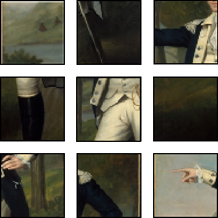
\includegraphics[width=0.4\textwidth]{30-part1/img/intro1.png}
    \hfill
    \subfloat{\qquad}
    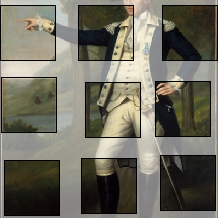
\includegraphics[width=0.4\textwidth]{30-part1/img/intro2.png}
    \caption[A task submitted to MTH1]{A task submitted to MTH1.}
    \label{fig:mth1:task}
\end{figure}

\blindtext

\paragraph{Sources}We walk through the following articles, presenting most of our contributions\footnote{The results are discussed in Chapter \ref{chap:res1}.}:
\begin{itemize}
    \item \href{https://hal.archives-ouvertes.fr/hal-01820489v2}{\publititle Jigsaw Puzzle Solving Using Local Feature Co-Occurrences in Deep Neural Networks};
    \item \href{https://hal.archives-ouvertes.fr/hal-01869765v2}{\publititle Image Reassembly Combining Deep Learning and Shortest Path Problem};
    \item \href{https://hal.archives-ouvertes.fr/hal-02494602v1}{\publititle Deepzzle: Solving Visual Jigsaw Puzzles with Deep Learning}.
\end{itemize}


% =======================================================

\section{Method overview}
\label{sec:mth1:ovw}

\blindtext

Our method addresses the following settings:
\blinditemize

We also …

% =======================================================

\section{Problem formulation}
\label{sec:mth1:formul}

Summary \blindtext

\paragraph{Notations} We introduce … .

\newthought{} Here is an equation without label:
\begin{equation*}
    \max P_r(x_c, x_{1,1}, x_{1,2}, \ldots, x_{2,j_1}, \ldots, x_{f,p}).
\end{equation*}

Here an equation with label:
\begin{equation}
    \label{eq:mth1:01}
    \max P_r(x_c, x_1, x_2, \ldots, x_f).
\end{equation}

% =======================================================

\section{Algorithms}
\label{sec:mth1:algo}

Algorithm \ref{algo:dz:greedy} presents the outline of the greedy solver:

\begin{algorithm}
    \caption[Greedy algorithm outline]{Greedy algorithm outline.}
    \label{algo:dz:greedy}
    \begin{algorithmic}[1]
        \Procedure{Greedy}{$Y$}
        \State $reassembly \gets [0] \times 8$
        \While{$0 \in reassembly$ \textbf{or} $Y \neq \emptyset$}
            \State $max\_frag, max\_pos \gets \text{argmax}(Y)$
            \State $reassembly[max\_pos] \gets max\_frag$
            \State $Y.\text{pop\_row}(max\_frag)$
            \State $Y.\text{pop\_column}(max\_pos)$
        \EndWhile
        \State \textbf{return} $reassembly$
        \EndProcedure
    \end{algorithmic}
\end{algorithm}
\newthought{}where $Y$ is …